\documentclass[tikz,border=10pt]{standalone}
\usepackage{amsmath}
\definecolor{bg}{HTML}{171D2B}
\definecolor{aksen}{HTML}{F7B538}
\definecolor{isibg}{HTML}{2A3550}
\begin{document}
\pagecolor{bg}
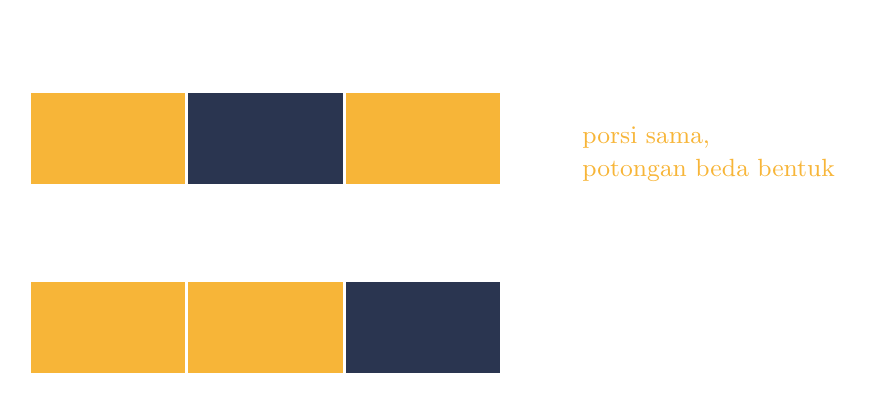
\begin{tikzpicture}[scale=1.0]
% Dua persegi panjang sama: 2/3 diarsir dengan arah beda
\begin{scope}
\fill[isibg] (0,0) rectangle (6,1.2);
\fill[aksen] (0,0) rectangle (2,1.2);
\fill[aksen] (4,0) rectangle (6,1.2);
\draw[white,line width=1.2pt] (0,0) rectangle (6,1.2);
\foreach \x in {2,4} \draw[white,line width=1.2pt] (\x,0) -- (\x,1.2);
\node[white,above] at (3,1.35) {$\frac{2}{3}$};
\end{scope}
\begin{scope}[yshift=-2.4cm]
\fill[isibg] (0,0) rectangle (6,1.2);
\fill[aksen] (0,0) rectangle (4,1.2);
\draw[white,line width=1.2pt] (0,0) rectangle (6,1.2);
\foreach \x in {2,4} \draw[white,line width=1.2pt] (\x,0) -- (\x,1.2);
\draw[white,line width=0.6pt,dashed] (2,0) -- (2,1.2);
\node[white,above] at (3,1.35) {$\frac{2}{3}$ juga};
\end{scope}
\node[aksen,right,align=left] at (6.9,0.4) {\small porsi sama,\\ \small potongan beda bentuk};
\end{tikzpicture}
\end{document}
